\chapter{Contribuição}\label{meto}

A contribuição dessa pesquisa é de cunho metodológico-prático.
Do ponto de vista metodológico, pela aplicação do processo CRISP-DM, usado para construir o modelo preditivo e classificativo; pela integração entre mineração de dados históricos e mineração de textos; pela utilização de uma multiplicidade de algoritmos: árvores de decisão, redes neurais, Naïve Bayes, TDF-IF, algoritmo Latent Dirichlet Allocation (LDA). Do ponto de vista prático, pela proposição de um modelo que integre predição à API de mapas de posicionamento global, fornecendo informação suficiente para um utilizador tomar uma decisão acerca dos dias e horários que ofereçam menor risco de acidentes ou qualquer evento que implique na retenção do fluxo de veículos. 

As soluções disponíveis que existem, tais como; Google Maps, Waze e outras ferramentas dessa natureza, somente exibem, até o momento dessa pesquisa, informações momentâneas, produzidas e compartilhadas pelos utilizadores dos aplicativos, ou por informações provindas de GPS. Contudo, não analisam dados históricos dessas rodovias, nem fazem predições sobre o seu comportamento.

Outra contribuição dessa pesquisa é a proposição de um arco cibernético construído com a API de redes sociais.
Os ``feeds'' de notícias das redes sociais como o Twitter permitem analisar o contexto das rodovias com defasagem temporal muito pequena.
Os utilizadores dessas redes sociais contribuem com informações relevantes como, por exemplo, o anúncio de uma paralisação que ocorrerá 
daqui a alguns dias. A PRF de Pernambuco é outro contribuidor permanente. Com seu canal no Twitter: @PRF191PE, fornece diariamente informação das rodovias, 
além de dados estatísticos de acidentes e retenção de tráfego. Os protestos, quando feitos dentro da lei
devem ser informados à PRF, com dia e hora marcados antecipadamente.

A monitoração de redes sociais é feita por Mineração de dados em textos, conhecida como Mineração em Textos ou "Text Mining" (TM).
A TM a princípio foi executada somente no Twitter no canal PRF191PE. 
Para ter-se acesso aos tweets da PRF, os usuários do canal, inclusive a própria PRF, postam comentários diretamente 
na API do Twitter ou por um navegador. Para nossa pesquisa as palavras-chave tais como: protestos, acidentes, paralisação, são de suma importância.

Uma vez capturados, esses tweets são tratadas por Mineração em Textos e analisados instantaneamente por algoritmos de I.A. 
A técnica utilizada para análise dos textos é análise de palavras ou termos frequentes (TDF-IDF). O algoritmo de classificação escolhido foi Naive Bayes, por ser um classificador rápido e eficiente, e por ter sido utilizado na primeira fase dessa pesquisa, servindo como comparativo à Árvore de Decisão. O algoritmo de agrupamento (clustering) foi o LDA.



\section{Modelo Proposto}

A metodologia utilizada nessa pesquisa contempla um plano em três etapas, cada uma dividida em fases atinentes.
A primeira etapa da nossa metodologia completa o ciclo todo do processo CRISP-DM, onde está o modelo classificativo, o preditivo e 
a descoberta de conhecimento sobre o comportamento das rodovias estudadas. A descoberta de conhecimento sobre esse comportamento 
 tem a ver com o ``modus operandi'' dos seus utilizadores. A priori, especulou-se sobre possíveis erros de traçados e outros que possam
ser identificados pelos algoritmos de mineração empregados no processo.

Os algoritmos escolhidos contemplaram algumas características especiais, tais como, robustez, tolerância à faltas (missing data),
taxa de aprendizagem e facilidade de interpretação dos dados processados. 

No quesito tolerância à faltas e facilidade de interpretação dos dados, a Árvore de Decisão e o Naïve Bayes se destacaram por não necessitar
de qualquer requisito extra para entender e interpretar os resultados.

No quesito robustez, tolerância à faltas e taxa de aprendizagem relativamente alta, as redes neurais artificiais (RNA), com a 
topologia Perceptron multicamadas com retroalimentação ``backpropagation'', se destacaram. 
As redes neurais têm capacidade de generalização e especificidade em modelos de predição. 

A extrapolação do modelo preditivo ocorre quando este se integra a uma estrutura dinâmica, composta pela redes sociais e mapas vetoriais, dado um espaço temporal pré-determinado por um agente: o utilizador. 

Através de API's, os mapas vetoriais permitem a geolocalização dos pontos classificados ou pontos onde haverá grande número de retenções, conhecido como \textbf{gargalo}.

A API do Twitter completa a informação, uma vez que o usuário informa, em seus tweets, a posição geográfica onde ocorrerá a paralisação, permitindo integração da estrutura
dinâmica com a preditiva.

Para a integração às redes sociais, foi escolhida a API do Twitter. Esta ``interface'' é simples de ser configurada. A quantidade de informações produzidas pelos utilizadores gera poucos dados em cada postagem, mas é eficaz. O utilizador tem que ser sucinto ao publicar suas postagem em um espaço de 140 caracteres. Isso facilita a forma como os dados são extraídos pela quantidade diminuta, bem como a quantidade de conexões à Internet. Contudo, esta rede social tem uma crescente quantidade de postagens no formato imagens, dificultando a mineração em textos. Esse aspecto foi particularmente relevante para essa pesquisa, quando foi constatado que a PRF também aumentou consideravelmente o número de tweets no formato de imagem. 

A alternativa escolhida para vencer essa dificuldade foi buscar conexões dos outros utilizadores do canal da PRF, uma vez que, as redes sociais, do ponto de vista tecnológico, se caracterizam como grafos e subgrafos interconectados, permitindo descobrir outras sub-redes que possivelmente conterão as informações desejadas. 

A figura a seguir ilustra (um overview) essa metodologia descrita graficamente.

\pagebreak

\begin{figure}[ht]
\centering
\caption{Etapas da modelo proposto}
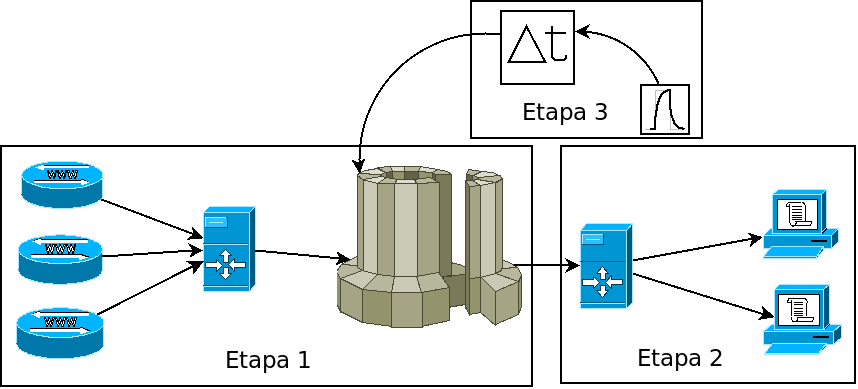
\includegraphics[width=170mm, height=85mm]{Figuras/Metodologia/metodologiaGeral.png}\\
\tiny Fonte: autor
\end{figure}

\section{Reflexão sobre as tecnologias utilizadas no modelo preditivo}\label{result}

Na fase de transformação de dados, da primeira etapa, onde são criadas novas variáveis, a proximidade entre as
bases heterogêneas foi conseguida utilizando regras de indução da lógica proposicional \cite{NorvigRussel2004}.
Nesta pesquisa, bases heterogêneas foram integralizadas em um único grande conjunto de dados, o ``data set''. As variáveis desse ``data set''são consideradas variáveis independentes, e foram preservadas aquelas com maior relevância ou as que continham a maior quantidade de conhecimento embutido, descoberto pelo cálculo da entropia. Foram também construídas novas variáveis, nas bases onde não havia correspondência, respeitando a lógica do negócio.\\
A tabela a seguir descreve as variáveis originais na base de dados de acidentes da PRF 

\pagebreak

\section{Extração do conhecimento - KDD}

O processo de descoberta do conhecimento iniciou-se com a coleta das bases de dados de acidentes da PRF. Optamos por coletar os dados dessa base diretamente na fonte,
ou seja dos servidores da PRF. Tais dados nos foram cedidos após alguns procedimentos burocráticos de praxe (ver anexos). Essa escolha foi motivada para tentar
mitigar o problema da qualidade dos dados. No artigo ``Uma análise da qualidade dos dados relativos aos boletins de ocorrências das rodovias federais para o processo de Mineração de Dados'' COSTA, BERNARDINI, LIMA et al (2012) destacam a não padronização e não aceitação dos dados pela comunidade internacional. EAVES, D. (2009) sugere que os dados sejam disponibilizados da maneira como foram coletados.

A PRF tem ao menos duas bases \footnote{Somente mencionamos bases de dados que interessaram à essa pesquisa.} de dados referentes às ocorrências nas rodovias BRs. A base de acidentes rodoviários e a base de intervenções que guarda as ocorrências que paralisaram as rodovias, tais como: protestos ou paralisações dessa natureza, feitos pelas pessoas que vivem no entorno das rodovias.

Para traçar um painel da diversidade das rodovias pernambucanas, foi efetuado a priori uma classificação através do algoritmo Árvore de Decisão e comparado com o classificador Naïve Bayes. Mediu-se a acurácia dos classificadores, comparando-se uma técnica algorítmica com a outra. A variável ``BRajustada'' mostrou ser a melhor variável para exprimir o nó raiz da Árvore de Decisão. Isso porque classificou os dados com o menor número de falsos positivos e com o maior número de verdadeiros positivos, obtendo curvas ROC com índices acima de 0.90. O Naïve Bayes também obteve índices de acurácia próximos a este, quando utilizado com o mesmo procedimento.

As técnicas como Redes Neurais Artificias (MLP) \cite{DecisaoCredito}, Árvores de decisão \cite{DataMining},  
 fornecem visão generalizada dos fatores preponderantes, levantando padrões ocultos nos dados. 


\section{Reflexão sobre as tecnologias utilizadas no modelo preditivo a posteriori}\label{resultPost}

ESCREVER....

\pagebreak

\section{Arco cibernético com dados do Twitter}

Os dados do Twitter, permite uma busca imediata por novas informações que poderão ser confrontadas com o 
modelo preditivo aumentando o nível de confiança deste, com isso a informação construirá um Arco cibernético, que segundo Wiener (1948) a 
informação permite realimentação aos sistemas, com controle mais eficaz, por exemplo: no trecho da Br 101, na altura do km 5, no 
Município de Goiana alguém publicou que a comunidade que mora no entorno dessa localidade fará um protesto daqui a dois dias devido ao 
acidente ocorrido ou a PRF publicou que o km 80 da Br 232, na altura do Município de Gravatá será interditada amanhã, por 2h, para 
remoção/explosão de rochas. 
Essas informações, por serem a posteriori às predições, podem aumentar o nível de confiança sugerida pelo modelo preditivo e controle por 
parte do utilizador e dentro de um universo temporal mais restrito servir de comprovação do das predições.

No entanto pode ocorrer o contrário quando as informações provenientes do modelo de predição entrar em conflito com as informações 
provenientes das redes sociais \footnote{O sistema de predição é baseado em cálculos probabilísticos}, para estes casos a decisão de 
qual ação a ser tomada sempre estará ``nas mãos'' do agente, o observador ou o utilizador.

As informações das redes sociais, armazenadas em um banco de dados, poderão servir futuramente para novas predições.
Essas informações que comporão o arco cibernético não deverão retroalimentar o modelo de predição já construído, pois o fluxo decisório
já foi tomado pelo observador, sendo que dados a posteriori não servem para um modelo de predição, enviesa o sistema preditivo.
Uma nova fase de Mineração de Dados, desta vez mineração de dados em textos com modelo de predição. 
Dessa forma compõe-se um novo arco cibernético, mais genérico à proposição inicial descrita.

\begin{figure}[ht]
	\centering
	\caption{O arco cibernético com o Twitter}
	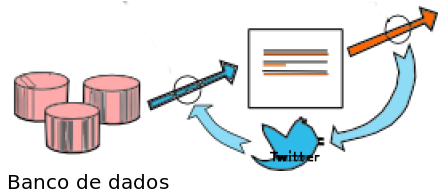
\includegraphics[width=90mm, height=45mm]{Figuras/Metodologia/ArcoCibernetico.png}\\
	\tiny Fonte: autor
\end{figure}

\pagebreak

\section{Extrapolação para georreferenciamento}

\begin{figure}[ht]
	\centering
	\caption{Etapas da metodologia}
	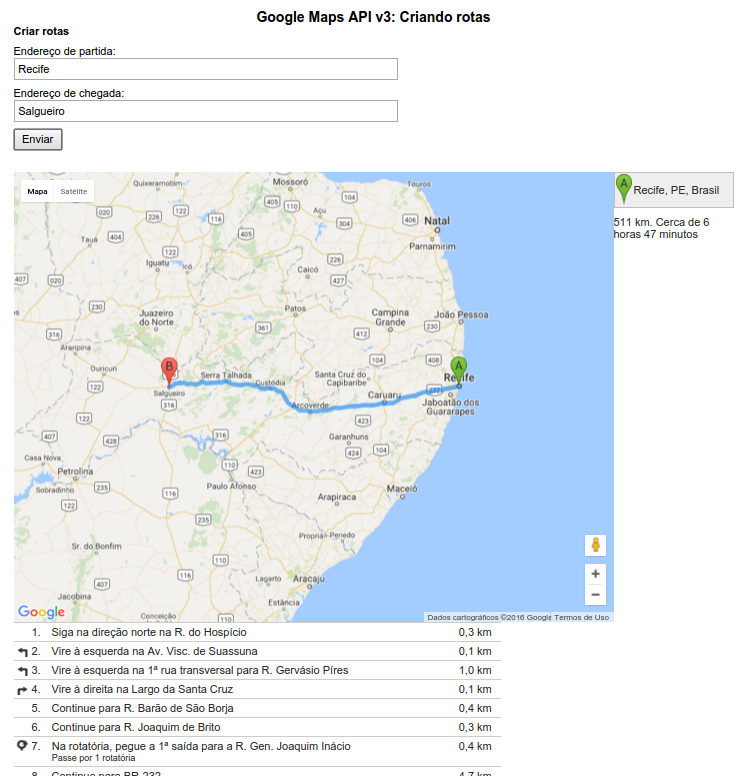
\includegraphics[width=150mm, height=130mm]{Figuras/Cronograma/GoogleMaps.png}
\end{figure}



